% Chapter 1

 % Write your own chapter title

\begingroup%
\makeatletter%
\let\clearpage\relax% Stop LaTeX from going to a new page; and
\vspace*{\fill}%
\vspace*{\dimexpr-50\p@-\baselineskip}% Remove the initial (default) 50pt gap (plus 1 line)
\chapterfont{\centering}
\chapter{Introduction}
\vspace*{\fill}%
\endgroup


\newpage
\label{Chapter1}
\lhead{Chapter 1. \emph{Introduction}} % Write in your own chapter title to set the page header

\section{Overview of the Project}
\justifying
We are making a Virtual Reality based E-commerce web application. This project is inspired by the meta-verse concept. The previous E-Commerce work never used any virtual stores or virtual environments in which different products were placed and customers can visit virtual stores in their homes just by wearing VR headsets. Currently, no website is having a virtual environment where customers can come with or without a VR headset and shop for wearable or other products just like they are shopping physically at the store. As for buying outerwear, customers have two options i.e to order online or to go to the mall or store. Another option is augmented reality in which the customer just opens up the camera and tries on different outfits \\ We will be catering to two types of customers, the ones having VR headsets will be able to visit the virtual store while wearing a VR headset where the customer can touch, and hold different products and can move in the virtual store. If the customer wants to try different outerwear like jackets so they can check the outerwear on their related Avatar in the virtual store and can experience it from all angles. Customers without VR headsets can visit the website and avail themselves of the virtual tour of the store where they don’t need any VR headsets. So basically, our modules consist of an E-commerce website, a Virtual tour environment, a Virtual Reality Environment that requires a VR headset, and proper and customized measurements of avatars and products so that customers can map them to themselves for a better virtual shopping experience.// Other than these, this application is providing advanced features to the customers like User-friendly navigation, Advanced Searching, Product Filtering, the Latest news section in which the latest discount and sales will be displayed to the customer, Conversion of currencies to different country’s currencies, etc.\\
\section{Background}
\justifying
In the previous already existing applications, implementation of the virtual reality mode of the E-commerce store was missing. It means the custosmers can see only the 2D images and lengthy descriptions of the product. Hence, there was a gap between the virtual and physical visits to the E-commerce store. Customers have to go to the store physically for a better experience of buying products. We overcome this situation by making an application in which we are going to implement 3D virtual reality mode and a 3D virtual tour of the E-commerce store integrated with the website having multiple features that every E-commerce website has. One huge feature that is going to be implemented is the customized product sizes for customers so that they can choose products according to their body measurements and requirements and experience this metaverse way of shopping to the next level.
\section{Problem Statement}
\justifying
There exists a huge gap between physical shopping and online shopping through web/mobile applications. To bridge the gap between the physical and digital worlds we are creating a virtual reality-based E-Commerce store that would provide a positive and realistic experience to the customers in the metaverse.
\section{Motivation}
\justifying
Our motivation is customer satisfaction by visiting the 3D virtual store in meta verse made with the latest technologies. Because there are lots of issues while visiting the shopping mall like time, conveyance issues, etc. So we are providing a positive digital virtual experience of shopping where customers with Oculus VR headsets can experience shopping that will be closer to real-time shopping in the shopping mall.\\
On the other hand, customers without VR headsets can do a virtual tour of the 3D E-commerce store. Based on customers’ body measurements, they can also map their sizes and choose a suitable product by customized measurements of avatars and other products.
\section{Objectives of the Project}
\justifying
Our objective is to remove the huge gap in the customer experience of online and physical shopping by introducing the virtual reality of the E-commerce store and providing real-time feeling to the customer with the help of a 3D virtual reality store and 3D Tour of virtual store. \\
The main objective is to create a VR-based E-commerce environment with the state of the art technologies to revolutionize the experience for online shopping experience for customers by introducing metaverse. One of our objectives is also to provide personalized customized fitting solutions for individual customers by introducing Meta-verse concepts and technologies.
\subsection{Industry Objective}
\justifying
Our industrial objective is to commercialize this application. This web application is to sell products in a virtual E-commerce store in Metaverse. But this application can be extended to other fields such as education, healthcare, etc. For example, some virtual online schools in our metaverse can be added. 
\subsection{Research Objectives}
\justifying
We are doing research on Meta verse concepts and how the real-world experience could be created in the digital world using advanced tools and technologies to provide customized/personalized fitting solutions according to the individual customers' body measurements. We are going to use our best knowledge and advanced technologies and frameworks  to make a virtual 3D store in meta verse as there exists no E-commerce system that provides a virtual reality-based online store with digital versions of the actual product, virtual avatars with different sizes, and customized positive experiences. Virtual reality with advanced technologies will shape the future of electronic retailing.\cite{MARTINEZNAVARRO2019475}
\subsection{Academic Objectives}
\justifying
The technologies and tools that we are using in our project will help us in our advanced learning and will fulfill our academic objectives as well.
\subsection{Business objectives}
\justifying
Following are some of the business objectives of the virtual reality-based e-commerce web application:
\begin{itemize}
    \item Profit maximisation
    \item Sales maximisation
    \item Revenue maximisation
    \item Surviving in the market
%    \item Satisficing principle
\end{itemize}
\section{Rules and assumptions}
Following are rules and cases of assumptions that are assumed to be true while experiencing virtual reality mode working:
\begin{itemize}
    \item The customer has an Oculus VR headset and the configurations/setting for Oculus VR Headset is also done by the customer before going into VR mode.
\end{itemize}
Following are rules and cases of assumptions that are assumed to be true while normally working:
\begin{itemize}
    \item The internet connection is stable.
\end{itemize}
\section{Scope of the Project}
\justifying
To bridge the gap between the physical and Digital worlds by creating a Virtual Reality-Based E-commerce Store that would provide positive and realistic experiences to customers in the metaverse. Currently, this application is limited to E-Commerce but this web application can be extended for virtual reality-based healthcare and educational systems.
\section{ Target Audience}
\justifying
Our Virtual reality-based e-commerce web application is dealing with average as well as professional customers. Professional customers who don't have much time to buy outerwear by going physically to shopping malls can just experience 3d virtual e-commerce stores for buying outerwear. On the other hand, average customers can do a 3D virtual tour of the e-commerce store. Those customers who don't know which size bests fits suits them can also avail of the best fitting size suggestion on our website.
\section{Challenges}
\subsection{VR Headset cost}
\justifying
The Oculus VR Headset price is about two lac that is not easily affordable by us and without this VR Headset, it's impossible to experience the virtual reality mode of the e-commerce store. So, buying VR Headset was one of the biggest challenges during the project working.
\subsection{Integration of Web-based and Unity Framework}
This was the second biggest challenge for us during the project. Because it was the first time for us when we were going to integrate the web with the unity and also the helping material for this was not available too much and the configurations of the VR Headset might affect the integration process.
\begin{figure}[H]
    \centering
    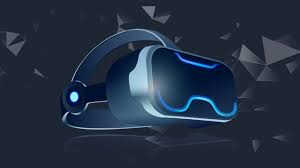
\includegraphics[width=15cm,height=10cm]{Figures/Others/VRHeadset.jpg}
    \caption{VR Headset}
    \label{VR HEeadset}
A head-mounted device used to experience virtual reality.  A hardware device that is connected to PC or mobile to experience VR environments and VR video games. VR headsets are mostly used in applications like trainers and simulators.
\end{figure}
\subsection{Configurations of VR Headset}
\justifying
To experience the virtual environment of unity in the oculus VR Headset we had to do configurations or settings in unity and it was not an easy task for us as after these configurations we were also going to integrate the unity environment with the Web.
\subsection{Understanding of payment API Integration}
\justifying
In our project, we used payment API for the first tie. It was quite difficult for us because this was the first time when we were going to integrate payment API in some web applications.
\subsection{Understanding how to integrate the processes}
\justifying
One of the challenges during project making was how to integrate the processes and what will be the sequence of the processes.
\subsection{Understanding of delivery method}
\justifying
One of the challenges was the understanding of the delivery method like when the customer order the product(i.e jacket) then the product should be delivered to the customer and on the successful delivery, we also need feedback from the customer. So handling all of this alone for us is difficult and we need a third party like Tcs etc for the delivery purpose the selection process for delivery and its API integration was also a big task for us.
\section{Constraints}
\justifying
The constraint of Virtual reality-based e-commerce web applications is that without VR headsets the customer cannot avail of the virtual reality mode. Because without an oculus VR headset the customer is unable to go into the 3D virtual store in meta verse but he can only do 3D of the store.
\section{Limitations}
This Virtual reality-based e-commerce web application is currently limited to clothes(only outerwear i.e jackets) only but it can be extended to further items that are part of future work.
etc.
Following are some of the limitations of our system as follow:
\begin{itemize}
    \item Our Virtual Reality based e-commerce store can work only on the desktop system, not on mobile phones or tablets, etc. 
    \item Real-time avatar creation through customer inputs is not currently implemented.
    \item Without a VR headset the virtual reality base e-commerce store cannot be experienced.
   % \item We had limited time to complete our project.
\end{itemize}

\section{Applications of Project}

\justifying
People can use this application to experience 3D virtual e-commerce at any place just by wearing an oculus VR headset. Without a VR headset customers can do a 3D tour of the store. Currently, our project is restricted to e-commerce only but it can be extended to various other fields as well like education, healthcare, buying and Decorating a House,
\section{Benefits of our Project to customer}

\justifying
Following are some of the possible applications of the virtual reality-based e-commerce web application:
\subsection{Better experience of buying a product online}
The customer without a VR headset like average customers can enjoy the 3D tour of the virtual 3D e-commerce store.
\subsection{Online 3D Tour facility}
The customer without a VR headset like average customers can enjoy the 3D tour of the virtual 3D e-commerce store.
\subsection{Ease to Customer}
This application will provide ease to the customer can experience the 3D virtual store by using an oculus VR headset at any location which can be home, office, etc. On the other hand, customers without an oculus VR Headset can also do a 3D virtual tour of the E-commerce store. The 3D images with 3D avatars will also give a realistic feeling to the customer and increase his/her engrossment.
\subsection{Customer Time Saving}
\justifying
It's a tedious task to go to a shopping mall and visit the whole store/mall to find your desired item. For example, you want to buy a jacket and you go to the mall and then visit the store to find your desired jacket. Let us suppose you did not find the desired one then you will have to return home and it's a real waste of time like you are wasting your time. Through this application, people can just experience a real-time 3D Virtual E-commerce store by using an oculus VR headset at any location which can be a home, office, etc.